\chapter{Z' Reconstruction}
\label{chap:reco}

The experimental signature in the search for long-lived $Z'$ is characterized by a high-$p_{T}$ dilepton vertex, displaced (>2 \si{\milli\meter}) from the primary vertex in transverse plane, referred a \textit{displaced vertex}. In this chapter, the reconstruction of displaced vertices in the ATLAS Inner Detector is described.

\section{Track Reconstruction in the Inner Detector}
\label{sec:reco:track}

Track reconstruction in the ATLAS uses pattern recognition algorithms to reconstruct the trajectories of charged particles, referred as \textit{track}. When a charged particle traverse through the ID, the particle interact with the sub-detectors of the ID (Pixel, SCT, and TRT), leaving raw detector signals. The raw signals are digitized and registered as detector \textit{hits}, and these detector hits are used for track reconstruction. 

\subsection{Standard Tracking}
\label{sec:reco:st}


\begin{figure}[!htb]
    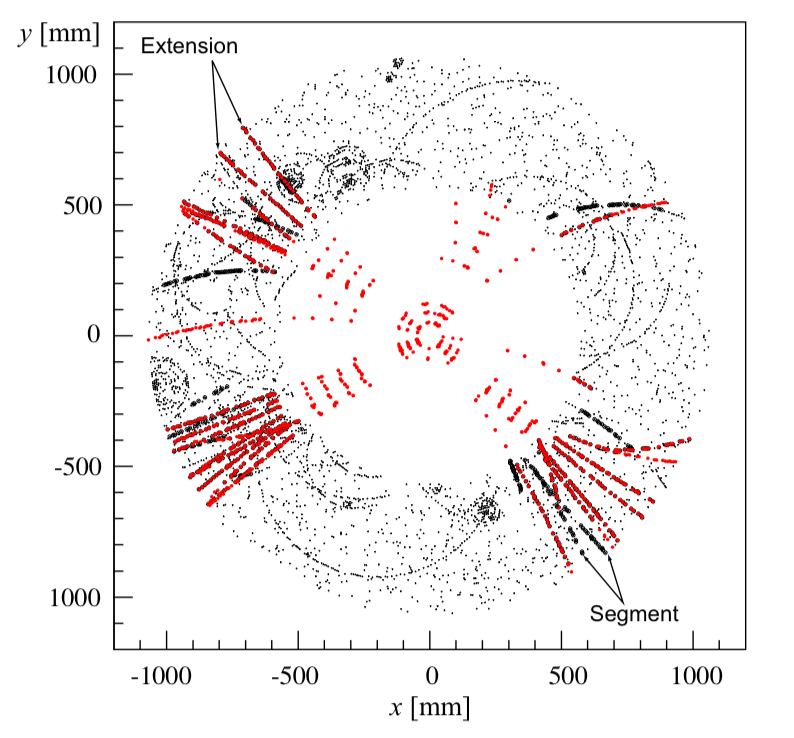
\includegraphics[width=0.6\textwidth]{figs/tracking.png}
    \centering
    \caption{Illustration of detector hits and reconstructed tracks in the Inner Detector. The bright colors represent the detector hits associated with reconstructed tracks~\cite{1742-6596-119-3-032014}.}
    \label{fig:tracking}
\end{figure}

The standard ATLAS track reconstruction is the main track reconstruction algorithm used in the ATLAS experiment. In the first stage of the track reconstruction, detector hits from the Pixel or the SCT detector are used to create \textit{track seeds}, collections of silicon hits used for the initial track finding. If a track seed passes certain quality criteria, including a $p_{T}$ and impact parameter selection, the track seed is extended to the outer part of the ID using a window search and pattern recognition algorithms. The extended tracks are evaluated based on $p_{T}$, number of hits, and impact parameters, and only the tracks satisfying the standard track selections are stored in the track collection. Figure~\ref{fig:tracking} illustrates detector hits and reconstructed tracks in the ID. The important standard track selections is summarized in Table~\ref{table:tracking}~\cite{ATL-PHYS-PUB-2017-014}.


Tracks are described by five parameters and a reference point, using a perigee representation. The parameters are the transverse (longitudinal) impact parameter $d_{0}$ ($z_{0}$), the azimuthal angle $\phi$, the polar angle $\theta$, and the charge-to-momentum ratio, $q/p$. The average position of the $pp$ interaction, referred as beamspot, is used as the reference point for the track representation~\cite{Aaboud:2016rmg}.


\begin{table}[!htb]
  \centering
  \begin{tabular}{ c  c  c }
    \hline
    & Standard & Large radius \\ [0.5ex]
    \hline
    Maximum $d_{\rm{0}}$ (mm) & 10 & 300 \\
    Maximum $z_{\rm{0}}$ (mm) & 250 & 1500 \\
    Maximum $|\eta|$ & 2.7 & 5 \\
    Maximum shared silicon modules & 1 & 2 \\
    Minimum unshared silicon hits& 6 & 5 \\
    Minimum silicon hits & 7 & 7\\
    Seed extension & Combinatorial & Sequential \\
    \hline
  \end{tabular}
  \caption{Important track selection in the standard and the large radius tracking algorithms.}
  \label{table:tracking}
\end{table}


\subsection{Large Radius Tracking}
\label{sec:reco:lrt}

The standard track reconstruction is proven to be very efficient in Run 2 with the tracking efficiency > 90\%~\cite{Aaboud:2017all}. However, the tracking algorithm is optimized for primary charged particles promptly produced from $pp$ collisions, and the strict requirements on the impact parameters, \dzero and \zzero potentially limit the tracking efficiency for the charged particles at large impact parameters ($d_{0}$ > 2 mm). Therefore, a dedicated track reconstruction algorithm, referred to as the large radius tracking (LRT), is developed to improve the track reconstruction efficiency for the tracks highly displaced from the primary vertex.

The LRT is performed in a sequence, following the standard tracking. It follows the same reconstruction strategy as the standard tracking, but there are a few importance difference between the standard tracking and the LRT.

\begin{itemize}
	\item The pattern recognition algorithms in the LRT only uses \textit{un-used} hits, the silicon hits that have not been used in the standard tracking, in creating and extending track candidates.
	\item The requirements on tracks such as $d_{0}$, $z_{0}$, and number of hits are relaxed.
\end{itemize}

The tracks satisfying certain criteria such as minimum $p_{T}$ and number of detector hits are merged into the track collection from the standard track reconstruction. The track selections in the LRT are summarized and compared with the standard track reconstruction in Table~\ref{table:tracking}. The combined track collection is used as an input for the lepton reconstruction and identification and secondary vertex reconstruction. More details on the large radius tracking can be found in Ref.~\cite{ATL-PHYS-PUB-2017-014}.

Combined with the standard track reconstruction, the LRT provides overall technical efficiency of $90\%$ or above for a displacement in the transverse plane up to 300 \si{\milli\meter}.


\section{Electron Reconstruction}
\label{sec:reco:lep}

Electrons are characterized by energy deposits in the EM calorimeter and the associated reconstructed tracks in the ID. The electron reconstruction algorithm uses the energy deposits with total transverse energy $>2.5$ \si{\GeV} in a window size of 0.075$\times$0.125 in ($\eta$,$\phi$) to reconstruct EM clusters. The EM clusters are associated with tracks within the same RoI with the requirement $|\Delta\eta|<0.05$ and $\Delta\phi$ where the effect of bremsstrahlung is taken into account. In the absence of a matching track, the EM cluster is classified as a photon candidate. The associated pairs of tracks and clusters are refitted to create electron candidates. Further electron requirements, including likelihood-based identification criteria, are imposed to the electron candidates for reconstructoin of electrons.

By default, electrons are required to have a minimum number of pixel hits and small transverse impact parameters. This is not optimal for the searches that aim to detect displaced vertices as the decay products of displaced vertices tend to have large impact parameters (\dzero, \zzero) and missing hits in the inner layers of the detector. Therefore, these requirements are removed in this analysis.

\section{Muon Reconstruction}
\label{sec:reco:muon}

Muons leave very small energy deposits in the calorimeter as they traverse through the detector due to the relatively larger mass, given that the probability of bremsstrahlung is $\propto 1/m^{2}$. However, they leave tracks in both the ID and the MS, referred as inner detector (ID) tracks and muon standalone (MS) tracks. The muon reconstruction algorithm uses MS tracks as seeds, and the MS tracks are extrapolated to the ID for the association with ID tracks. A \textit{combined muon} track is created if a MS track is successfully associated with an ID track after the momentum correction for the energy loss from the interaction with the detector material. There are other types of reconstructed muons such as standalone muons, segment-tagged muons, and calorimeter-tagged muons~\cite{Aad:2016jkr}. However, these types of muons are not considered in this analysis as they do not have associated ID tracks which are required for the reconstruction of displaced vertices.

Similar to electrons, the requirements on a minimum number of pixel hits and minimum impact parameters (\dzero, \zzero) are removed in this analysis.


\section{Secondary Vertex Reconstruction}
\label{sec:reco:dv}

\begin{figure}[!htb]
    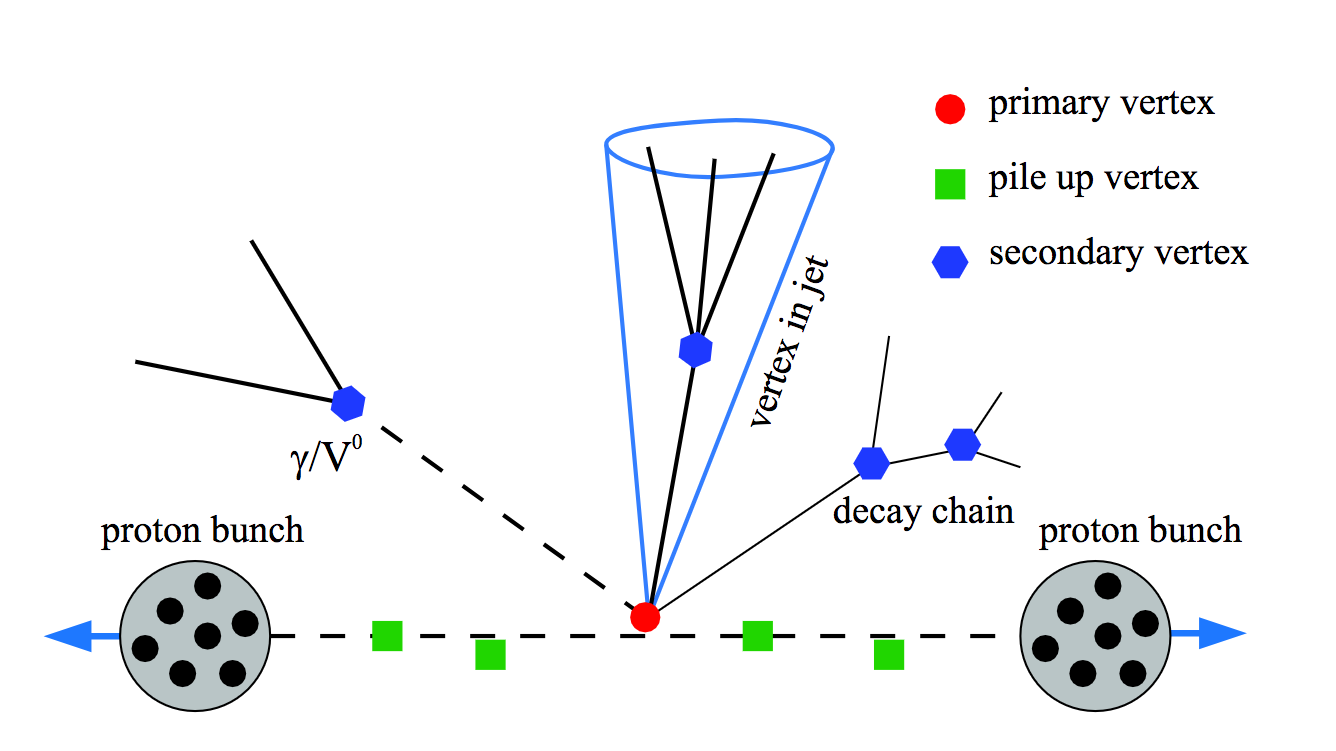
\includegraphics[width=0.6\textwidth]{figs/vertex.png}
    \centering
    \caption{Important vertex topologies in $pp$ collisions: primary, pile-up, and secondary vertices.}
    \label{fig:vertex_topology}
\end{figure}

In the LHC, when two proton bunches collide, several different vertex topologies arise. The primary vertex and several pile-up vertices are formed along the beam line, and the vertices from photon conversion or long-lived particles are formed displaced from the primary vertex as shown in Figure~\ref{fig:vertex_topology}. These displaced vertices are referred as secondary vertices. In the search for long-lived $Z'$ in dilepton decay channel, the decay products of long-lived particles can be reconstructed as a secondary vertex.

The secondary vertex reconstruction is based on the algorithm developed for the primary vertex reconstruction~\cite{1742-6596-119-3-032033}. In the first stage of the secondary vertex reconstruction, track are selected using the requirements on track parameters and hit patterns shown in Table~\ref{table:vertex_track_selection_simple}. The tracks reconstructed by both the standard track reconstruction and the LRT are used as input. The tracks passing the track requirements are used to create two-track vertices, based on the closeness of two tracks in the space. This process results in a large number of fake vertices. The fake vertices are rejected by considering the location of a vertex and hit patterns of the tracks associated with the vertex. A vertex is rejected if the associated tracks have any hits at a radius smaller than the vertex position. Two-track vertices passing the fake rejection are refitted using a Kalman Filter for precise vertex position measurements, and track parameters are calculated with respect to the secondary vertex.

The two-track vertices reconstructed by the secondary vertex reconstruction serves as the primary analysis object in this thesis. 


\begin{table}[!htb]
  \centering
  \begin{tabular}{ l c }
    \hline
    \hline
	Variable      		& Cut                                         	\\
    \hline
	$p_{T}$ (GeV)		& $>$ 1.0										\\
	$\chi^{2} / DOF$	& $<$ 50.0										\\
	$d_{0}$	(mm)		& 2.0 - 300.0									\\
	$z_{0}$ (mm)		& $<$ 1500.0									\\
	SCT hits			& $\geq$ 2										\\
	Si shared hits	    & $\leq$ 2										\\
	Pixel and TRT hits  & TRT hits > 0 or Pixel hits $\geq$ 2			\\
    \hline
    \hline
  \end{tabular}
  \caption{Track requirements for secondary vertex reconstruction.}
  \label{table:vertex_track_selection_simple}
\end{table}


